\chapter{Design of the System} \label{chap:design}
The design of the system is expressed in this chapter through explanation of the components used in the Fog Computing based face identification system. Practical details of implementing this design are covered in the next chapter.

\section{Overview}
On the whole, the system consists of two behaviour mode, namely off-peak mode and peak mode. Off-peak mode means the requests from end devices are sparse or distributed evenly so that Fog Nodes own the capability of responding within a limited time slot. Cloud Nodes are not involved in this mode. On the contrary, peak mode demands the power of Cloud Nodes. This mode relies on a dynamic allocation mechanism which monitors the pressure of the Fog Nodes.

\section{Off-peak Mode}
This mode only cover the lower two layers in the figure \ref{fig:design_of_the_system}. As you can see in the figure, the lowest layer contains end devices in the network of the Internet of Things. 

In the implementation, The Nexus 6 Android phone is used to play the role of the end device. Though there is only one android depicted in the figure, it is on behalf of all Internet of Things devices with limited hardware resource. This device is in charge of collecting images through preview frame from a camera and sending them to a closest working Fog Node periodically.

The Fog Nodes in the higher layer (medium layer) substitute the Cloud counterparts as the resource pool of computing. They are commodity personal computers in the implementation. They provide the service of face detection and face recognition. At the same time, they monitor the traffic of request to make the decision that whether Cloud Nodes should be included in the computing cycle and how many of them are required. This feature is called dynamic allocation in the system.

\section{Peak Mode}
Peak mode contains three layers as a whole. Compared to off-peak mode, one more layer is added. The top layer consists of Cloud Nodes, and the rest of layers are the same with the off-peak mode.

Peak mode is activated when the requests from the end devices are frequent. This mode involves Cloud Nodes, which make it different from the Fog mode. Amazon EC2 or other cloud computing infrastructures are used as an elastic resource pool. Due to its characteristic of elasticity, temporary high demand for computing tasks can be flattened.

Expected disadvantages of introducing the Cloud Nodes includes longer latency and security issues.

\section{Face Identification}
Face detection and recognition algorithm themselves are popular research topics. Consider they are not the focal topic of this research, popular algorithms are implemented to gain confidence for the system.

\begin{figure}
    \centering
    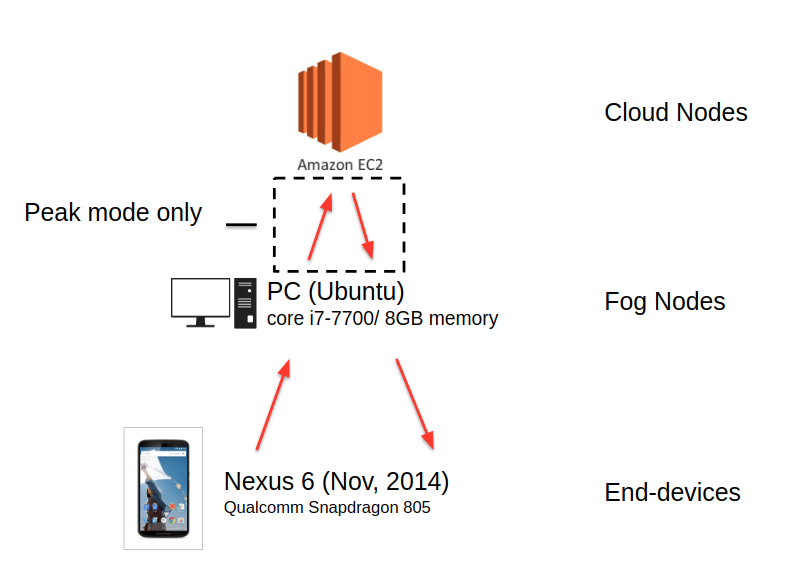
\includegraphics[width=0.7\textwidth]{images/design-of-the-system.png}
    \caption{Design of the System}
    \label{fig:design_of_the_system}
\end{figure}

